\documentclass[a4paper]{article}

\usepackage[italian]{babel}
\usepackage{algorithmic}
\usepackage{amsmath}
\usepackage{amssymb}
\usepackage{amsthm}
\usepackage{graphicx}
\usepackage[colorlinks=true, allcolors=blue]{hyperref}
\usepackage{bookmark}
\usepackage{biblatex}
\usepackage{csquotes}
\usepackage{nicefrac}
\usepackage{leftindex}
\usepackage{float}
\usepackage{booktabs}
\usepackage{multirow}
\usepackage{multicol}

\usepackage{matlab-prettifier}

\renewcommand{\lstlistingname}{Codice}

%% Since I want "Input" and "Output" in the algorithm, I will need
\usepackage{algorithm}
\renewcommand{\algorithmicrequire}{\textbf{Input:}}
\renewcommand{\algorithmicensure}{\textbf{Output:}}

\makeatletter
\renewcommand{\ALG@name}{Algoritmo}
\makeatother

% Since I will write algorithm in two columns, I will need
\usepackage{multicol}

\newcommand{\dist}{{\rm dist}}
\newcommand{\NN}{\mathbb{N}}
\newcommand{\NNp}{\mathbb{N}_{> 0}}
\newcommand{\RR}{\mathbb{R}}
\newcommand{\CC}{\mathbb{C}}
\DeclareMathOperator*{\argmin}{\arg\!\min}
\DeclareMathOperator*{\argmax}{\arg\!max}
\newcommand{\evec}{{\bf e}}
\newcommand{\cvec}{{\bf c}}
\newcommand{\avec}{{\bf a}}
\newcommand{\qvec}{{\bf q}}
\newcommand{\vvec}{{\bf v}}
\newcommand{\uvec}{{\bf u}}
\newcommand{\xvec}{{\bf x}}
\newcommand{\bone}{\mathbf{1}}
\newcommand{\bzero}{{\bf 0}}
\newcommand{\inv}{^{-1}}
\newcommand{\cS}{\mathcal{S}}
\newcommand{\cE}{\mathcal{E}}
\newcommand{\cEout}{\cE^\text{out}}
\newcommand{\cEin}{\cE^\text{in}}
\newcommand{\cN}{\mathcal{N}}
\newcommand{\cF}{\mathcal{F}}

\DeclareMathOperator{\nnz}{nnz}
\DeclareMathOperator{\rk}{rk}
\DeclareMathOperator{\tr}{tr}

\newcommand{\se}{\text{se }}
\newcommand{\altrimenti}{\text{altrimenti}}

\newcommand{\OO}{\mathcal{O}}

\newtheorem{theorem}{Teorema}
\newtheorem{lemma}{Lemma}
\newtheorem{definition}{Definizione}
\newtheorem{remark}{Osservazione}
\newtheorem{proposition}{Proposizione}
\newtheorem{corollary}{Corollario}

\addbibresource{biblio.bib}

\usepackage{chngcntr}
\counterwithout{table}{section} 
\renewcommand{\thetable}{\arabic{table}}

\title{Implementazione di un algoritmo per il calcolo efficiente del ranking dato dalla centralità di Katz in grafi molto densi}
\author{Gabriel Antonio Videtta (\textsc{654839})}

\begin{document}
\maketitle

\begin{abstract}
In questa relazione presentiamo la teoria e gli algoritmi
proposti da \cite{katz2024} per calcolare efficientemente il ranking indotto dal
vettore di Katz in grafi molto densi sfruttando la nozione di ``grafo complementare''
e dando significato al calcolo di indici di centralità di Katz con parametri
negativi.
\end{abstract}

\section{Prerequisiti teorici}

Ricordiamo brevemente che un grafo (eventualmente \textit{con lacci}) è una coppia di insiemi $G = (V, E)$ con $E \subseteq V \times V$ e $V = \{1, \ldots, n\}$ per qualche $n \in \NNp$. Gli elementi dell'insieme $V$ sono detti \textit{nodi}, mentre quelli dell'insieme $E$ sono detti \textit{archi}.

Quando si parla di grafi \textit{senza lacci} (o di grafo \textit{semplice}), si esclude a priori l'esistenza di archi
della forma $(i, i)$ con $i \in V$.

Nel corso della relazione useremo $n$ per riferirci al numero di
nodi del grafo preso in considerazione, e useremo $m$ per riferirci al
numero di archi dello stesso.

L'insieme $E$ induce una relazione $\sim$ su $V$ tale per cui $i \sim j$ se e solo se $(i, j) \in E$. Il grafo $G$ si dice \textit{non orientato} se $\sim$ è simmetrica, e \textit{orientato} altrimenti.

Un sottografo di $G$ è un grafo $G' = (V', E')$ con $V' \subseteq V$
e $E' \subseteq (V' \times V') \cap E$.

Un grafo è rappresentato operativamente tramite la propria \textit{matrice
di adiacenza} $A \in \RR^{n \times n}$, definita componente per componente come
\[
    A_{ij} = \begin{cases}
        1 & \se i \sim j, \\
        0 & \altrimenti.
    \end{cases}
\]

Si osserva immediatamente che $A$ è simmetrica se e solo se $G$ è non orientato.

Un grafo è detto \textit{sparso} se $A$ ha $\OO(n)$ entrate non nulle, mentre è detto \textit{denso}
se tutte le entrate di $A$ eccetto per un numero $\OO(n)$ di queste sono non nulle. Equivalentemente, un grafo sparso è tale per cui $m = \OO(n)$.

Un \textit{cammino orientato} (\textit{directed walk} in inglese) di lunghezza $r$ dal nodo $i$ al nodo $j$ è una sequenza
ordinata di $r+1$ nodi $i_0 = i$, $i_1$, ..., $i_r = j$ dove $i_k \sim i_{k+1}$ per ogni $k = 0$, $1$, ..., $r-1$.

Un \textit{cammino non orientato} (\textit{undirected walk} in inglese) ignora le direzioni, ovverosia permette di passare da $i$ a $j$
anche se $j \sim i$.

Nel caso di un grafo non orientato, si identificano cammini orientati
e non orientati, chiamandoli entrambi semplicemente \textit{cammini}.

Un cammino (orientato o non orientato) è detto \textit{elementare} (\textit{path} in inglese) se ogni nodo è toccato al più una volta.

Un grafo è detto \textit{connesso} se dati due nodi esiste sempre un cammino non orientato che li collega, mentre è detto \textit{fortemente connesso} se dati due nodi esiste sempre un cammino
orientato che li collega. Un grafo non orientato è connesso se e solo se è fortemente connesso, dal momento che cammini orientati e non orientati sono
identificati. Un grafo è fortemente connesso se e solo se la sua matrice di adiacenza è
irriducibile per permutazioni (vd. \cite[Theorem 3.2.1]{brualdi1991combinatorial}).

Si dice \textit{componente connessa} del nodo $i$ il più grande sottografo
connesso di $G$ contenente $i$. Analogamente si definisce una \textit{componente fortemente connessa}. 

Nel corso di questa relazione, scriveremo
$\bone \in \RR^n$ per riferirci al vettore composto da soli uno, $\bzero \in \RR^n$ per riferirci al vettore nullo, $I \in \RR^{n \times n}$ per riferirci
alla matrice identità e $\evec_k \in \RR^n$ per riferirci alla $k$-esima colonna di $I$. Scriveremo $\avec_k$ per riferirci alla $k$-esima colonna di una matrice $A$ e $a_k$ per riferirci al $k$-esimo elemento di un vettore $\avec$.

\subsection{Il vettore di Katz e buona definizione}

Ricordiamo un altro classico risultato della teoria dei grafi, facilmente
dimostrabile per induzione.

\begin{lemma}
    \label{lemma:numero_cammini}
    Sia $A$ la matrice di adiacenza di un grafo $G$ e sia $r \in \NN$. Allora l'entrata $(i,j)$-esima di $A^r$ rappresenta il numero di cammini
    di lunghezza $r$ da $i$ a $j$.
\end{lemma}

\begin{remark}
    \label{remark:molt_per_1}
    Dal Lemma~\ref{lemma:numero_cammini} segue facilmente che l'$i$-esima
    coordinata del vettore $A^r \bone$ rappresenta il numero di cammini
    di lunghezza $r$ che partono da $i$ e che terminano in un qualsiasi nodo.
\end{remark}

\begin{definition} Se $\alpha \in (-\nicefrac{1}{\rho(A)}, \nicefrac{1}{\rho(A)})$\footnote{Il limite superiore $\nicefrac{1}{\rho(A)}$ è necessario affinché la serie converga a $(I-\alpha A)\inv$.}, {\rm il vettore di Katz in $\alpha$ di $A$} è definito come il vettore
\[
    \xvec := (I + \alpha A + \alpha^2A^2+\cdots) \bone = (I-\alpha A)\inv \bone.
\]

Equivalentemente, $\xvec$ è l'unica soluzione del sistema lineare $(I-\alpha A)\xvec = \bone$.
\end{definition}

\begin{remark}
    Se $\alpha > 0$, il vettore di Katz induce un naturale ranking dei nodi di $G$, dove l'importanza
    di un nodo $i$ è determinata dai cammini che hanno sorgente $i$: a
    un cammino di lunghezza $r$ è associato un valore $\alpha^r$,
    e sommando tutti questi valori si ottiene la coordinata di $i$
    nel vettore di Katz.

    Nella teoria si vorrebbe che $\alpha^r$ decresca all'aumentare di $r$,
    ovverosia che i cammini più lunghi abbiano sempre meno importanza.
    Questo non è immediatamente ovvio, dal momento che $\nicefrac{1}{\rho(A)}$ potrebbe essere maggiore di $1$. La {\rm Proposizione
    \ref{prop:spectral_radius}} mostra che $\rho(A) > 1$ nella maggior
    parte dei casi considerati, garantendoci di star dando la giusta
    interpretazione alla costruzione del vettore di Katz.
\end{remark}

\begin{definition}
    Se $G$ è un grafo non orientato, si definisce {\rm grado} $\deg(i)$
    del nodo $i$ il numero di archi insistenti su $i$. Equivalentemente
    $\deg(i) = \bone^T A \mathbf{e}_i$.
\end{definition}

\begin{lemma}[Handshaking lemma]
    \label{lemma:handshake}
    Se $G$ è un grafo semplice non orientato, allora
    \[ \sum_{i \in V} \deg(i) = 2m. \]
\end{lemma}

\begin{proof}
    Si tratta di una semplice verifica combinatoriale:
    \begin{eqnarray}
        \sum_{i \in V} \deg(i)
        &=& \sum_{i \in V} \bone^T A \mathbf{e}_i \nonumber \\
        &=& \bone^T A \bone \nonumber \\
        &=& 2m, \nonumber
    \end{eqnarray}
    dove si è usato che non esistono lacci in $G$ e che gli elementi
    non nulli di $A$ sono tanti quanto il doppio degli archi in $G$.
\end{proof}

\begin{definition}
    Se $G$ è un grafo non orientato, si definisce {\rm il grado medio} $d_G$ di $G$ come
    la media dei gradi dei nodi, ovverosia
    \[
        d_G = \frac{\sum_{i \in G} \deg(i)}{n}.
    \]
\end{definition}

\begin{proposition}
    \label{prop:spectral_radius}
    Se un grafo semplice non orientato $G$ ha almeno un nodo con grado almeno $2$ e $A \in \RR^{n \times n}$ è la sua matrice di adiacenza, allora $\rho(A) > 1$.
\end{proposition}

\begin{proof}
    Sia $C$ una componente connessa di $G$ a cui appartiene almeno un nodo
    di grado almeno $2$, e indichiamo con $V(C)$ l'insieme dei nodi di $C$,
    con $n_C$ il numero di nodi $|V(C)|$ e con $m_C$ il numero di archi di $C$. Sia $\evec_C$ il vettore indicatore dei membri di $C$, ovvero tale che
    \[
        (e_C)_i = \begin{cases}
            1 & \se i \in V(C), \\
            0 & \altrimenti.
        \end{cases} 
    \]
    Allora $\evec_C^T \evec = n_C$, il numero di nodi nella componente $C$, mentre vale che
    \[
        \evec_C^T A \evec_C = \sum_{i \in C} \deg(C) = 2 \cdot m_C
    \]
    dove $m_C$ è il numero
    degli archi in $C$
    e l'ultima uguaglianza è data dal Lemma \ref{lemma:handshake}. Dal momento che $C$ è connesso, allora $C$ deve contenere almeno $n_C-1$ archi, ovverosia
    $m_C \geq n_C - 1$. Se $d_C$ è il grado medio di $C$, allora:
    \[
        d_C = \frac{\evec_C^T A \evec_C}{\evec_C^T \evec_C} \geq \frac{2(n_C-1)}{n_C} \geq \frac{4}{3},
    \]
    dove nell'ultima disuguaglianza si è sfruttato che $n_C \geq 3$, dal momento che
    esiste almeno un nodo in $C$ di grado $2$.

    Poiché $A$ è una matrice simmetrica reale, $\rho(A)$ maggiora
    sicuramente $d_C$, che è il
    quoziente di Rayleigh per la matrice $A$ e il vettore $e_C$ (vd. \cite[Theorem 4.4.2]{friedland2015}),
    e pertanto $\rho(A) \geq \frac{4}{3} > 1$.
\end{proof}

\section{Grafo complementare e vettore di Katz}

In questa sezione della relazione, presentiamo il concetto di grafo
complementare, eventualmente senza lacci, e tramite i Teoremi
\ref{th:compl_1} e \ref{th:compl_2}, preceduti dai preziosi Lemmi
\ref{lemma:matrix_determinant_lemma} e \ref{lemma:sherman},
troviamo una corrispondenza che ci permette di calcolare il vettore di
Katz sul grafo complementare, ottenendo lo stesso ranking che avremmo
ottenuto calcolandolo sul grafo originale.

\begin{definition}
    Su un grafo (con eventualmente lacci) $G = (V, E)$ si definisce il {\rm \textbf{grafo complementare}}
    $G^c = (V, E^c)$ come il grafo tale per cui $E^c$ è il complementare di $E$ in $V \times V$.


    Su un grafo senza lacci $G = (V, E)$ si definisce il {\rm \textbf{grafo complementare senza lacci}} come il grafo complementare di $G$ a cui
    si tolgono i lacci.
\end{definition}

\begin{remark}
    La matrice di adiacenza di un grafo complementare si ottiene come
    una modifica di rango $1$ della matrice di adiacenza di partenza (cambiata di segno), ovverosia, se $A^C$ è la matrice di adiacenza
    del complementare e $A$ è la matrice di adiacenza originale vale
    \[
        A^C = \evec \evec^T - A.
    \]
    La matrice di adiacenza di un grafo complementare senza lacci si
    ottiene invece come una modifica di rango $1$ su $A+I$ (cambiata
    di segno):
    \[
        A^{CC} = \evec \evec^T - A - I
    \]
\end{remark}

\begin{lemma}
    \label{lemma:matrix_determinant_lemma}
    Sia $A \in \CC^{n \times n}$ una matrice invertibile e siano $\uvec$ e $\vvec$ vettori in
    $\CC^n$. Allora $\det(A + \uvec \vvec^T) = \det(A) (1+\vvec^TA^{-1}\uvec)$.
\end{lemma}

\begin{proof}
    Dimostriamo innanzitutto il lemma nel caso in cui $A = I$.
    
    Poiché
    $\uvec \vvec^T$ è una matrice di rango $1$, $\uvec \vvec^T$ ha come autovalore $0$ con
    almeno molteplicità $n-1$. L'unico altro autovalore, che è eventualmente $0$,
    è allora $\tr(\uvec \vvec^T)$, ovverosia $\vvec^T \uvec$. Pertanto il polinomio caratteristico
    di $\uvec \vvec^T$ risulta essere
    \[p_{\uvec \vvec^T}(t) = \det(\uvec \vvec^T - tI) = (-1)^{n} t^{n-1}(t-\vvec^T \uvec).\]

    Dunque, $\det(I+\uvec \vvec^T) = \det(\uvec \vvec^T - (-1)\cdot I) = 1+\vvec^T \uvec$,
    dimostrando il caso in cui $A = I$. 
    
    Nel caso generale, considerato che $A + \uvec \vvec^T = A(I+A^{-1}\uvec \vvec^T)$, applicando l'identità di Binet si ottiene
    \[
        \det(A + \uvec \vvec^T) =
        \det(A) \det(I + A^{-1} \uvec \vvec^T) = \det(A) (1+\vvec^T A^{-1} \uvec),
    \]
    completando la dimostrazione.
\end{proof}

\begin{lemma}[Sherman-Morrison]
    \label{lemma:sherman}
    Se $A \in \CC^{n \times n}$ è invertibile e $\uvec$ e $\vvec$ sono vettori in $\CC^n$, allora $A + \uvec \vvec^T$ è invertibile se e solo se $1 + \vvec^T A^{-1} \uvec$ è diverso da $0$, e in tal caso vale che
    \[
        (A+\uvec \vvec^T)^{-1} = A^{-1} - \frac{A^{-1} \uvec \vvec^T A^{-1}}{1 + \vvec^T A^{-1} \uvec}.
    \]
\end{lemma}

\begin{proof}
    La prima parte del lemma è un corollario del Lemma \ref{lemma:matrix_determinant_lemma}.
    La seconda parte è una semplice verifica diretta:
    \begin{eqnarray}
        (A+\uvec \vvec^T)\left(A^{-1} - \frac{A^{-1} \uvec \vvec^T A^{-1}}{1 + \vvec^T A^{-1} \uvec}\right)
        &=&
        I+\uvec \vvec^TA^{-1} - \frac{\uvec \vvec^TA^{-1} + \uvec \vvec^T A^{-1} \uvec \vvec^T A^{-1}}{1 + \vvec^T A^{-1} \uvec} \nonumber \\
        &=& I+\uvec \vvec^TA^{-1} - \frac{(1+\vvec^T A^{-1} \uvec)\uvec \vvec^TA^{-1}}{1+\vvec^T A^{-1} \uvec} \nonumber \\
        &=& I + \uvec \vvec^T A^{-1} - \uvec \vvec^TA^{-1} \nonumber \\
        &=& I. \nonumber
    \end{eqnarray}
\end{proof}

\begin{theorem}
    \label{th:compl_1}
    Sia $G$ un grafo. Se $\alpha \in (0, \nicefrac{1}{\rho(A)})$, allora il vettore di Katz di parametro $-\alpha$ calcolato sul complementare (con lacci) $G^C$
    induce lo stesso ranking del vettore di Katz di parametro $\alpha$ calcolato su $G$.
\end{theorem}

\begin{proof}
    Innanzitutto, osserviamo che
    \[ I+\alpha A^C = (I-\alpha A)+\alpha \evec \evec^T. \]
    Pertanto, per il Lemma \ref{lemma:matrix_determinant_lemma},
    $I + \alpha A^C$ è invertibile se e solo se
    \[ 1 + \alpha \evec^T (I - \alpha A)^{-1} \evec \neq 0. \]
    Dal momento che $\alpha > 0$, il termine $\alpha \evec^T (I - \alpha A)^{-1} \evec$ è certamente positivo, e dunque $I + \alpha A^C$ è invertibile.

    Sia $A$ la matrice di adiacenza di $G$. Allora la matrice di adiacenza
    $A^C$ di $G^C$ è tale per cui $A^C = \evec \evec^T - A$. Si osserva
    che, per il Lemma \ref{lemma:sherman}, vale che
    \begin{eqnarray}
        (I-\alpha A)^{-1}
        &=& (I - \alpha (\evec \evec^T - A^C))^{-1} \nonumber \\
        &=& (I+\alpha A^C-\alpha \evec \evec^T)^{-1} \nonumber \\
        &=& (I + \alpha A^C)^{-1} - \frac{(I + \alpha A^C)^{-1} (-\alpha \evec \evec^T) (I + \alpha A^C)^{-1}}{1 + \evec^T (I + \alpha A^C)^{-1} (-\alpha \evec)} \nonumber \\
        &=& (I + \alpha A^C)^{-1} + \alpha \frac{(I + \alpha A^C)^{-1} \evec \evec^T (I + \alpha A^C)^{-1}}{1 - \alpha \evec^T (I + \alpha A^C)^{-1} \evec}. \label{eq:first_step}
    \end{eqnarray}

    Sia $\gamma$ definito come
    \[
        \gamma = \evec^T (I + \alpha A^C)^{-1} \evec.
    \]

    Allora, grazie all'eq.~\eqref{eq:first_step}, il vettore di Katz di $A$ si riscrive come
    \begin{equation}
        \label{eq:second_step}
        (I-\alpha A)^{-1} \evec = \frac{1}{1 - \alpha \gamma} \, (I + \alpha A^C)^{-1} \evec.
    \end{equation}

    Dall'eq.~\eqref{eq:second_step} si ricava inoltre che
    \begin{equation} \label{eq:third_step}
        (I + \alpha A^C) (I-\alpha A)^{-1} \evec = \frac{1}{1 - \alpha \gamma} \, \evec.
    \end{equation}

    Poiché il termine $(I + \alpha A^C) (I-\alpha A)^{-1} \evec$ dell'eq.~\eqref{eq:third_step} è non negativo, allora
    anche il termine a destra è non negativo, da cui
    $1 - \alpha \gamma > 0$, e dunque $\alpha \gamma < 1$.

    Pertanto $(I + \alpha A^C)^{-1} \evec$, che è proporzionale a $(I-\alpha A)^{-1} \evec$ per un fattore positivo per
    l'eq.~\eqref{eq:second_step}, è un vettore non negativo ed induce correttamente un ranking dei nodi equivalente
    a quello generato dal vettore di Katz di $A$.
\end{proof}

\begin{theorem}
    \label{th:compl_2}
    Sia $G$ un grafo. Se $\alpha \in (0, \nicefrac{1}{\rho(A)})$, allora il vettore di Katz di parametro $-\frac{\alpha}{1+\alpha}$ calcolato sul complementare senza lacci $G^C$
    induce lo stesso ranking del vettore di Katz di parametro $\alpha$ calcolato su $G$.
\end{theorem}

\begin{proof}
    La dimostrazione segue pressoché gli stessi passaggi della dimostrazione del Teorema \ref{th:compl_1} definendo
    $A^{CC} = \evec \evec^T - (A+I)$ al posto di $A^C = \evec \evec^T - A$.
\end{proof}

\section{Sperimentazione numerica}

Le simulazioni sono state eseguite in ambiente MATLAB R2024b su un PC desktop equipaggiato con 32 GB di RAM e
processore Intel i7-10700K con un clock rate di 3.80 GHz. Tutti i codici sono inclusi anche in \cite{hearotCode}.

\subsection{Generazione dei grafi}

Prima di implementare operativamente il calcolo del vettore di Katz mediante il grafo complementare, si è innanzitutto scritto
una funzione che, dato un parametro $d$, genera un grafo senza lacci, non diretto e denso di densità $d$ (Codice \ref{code:dense_graph}).

\begin{figure}[H]
    \centering
    \begin{lstlisting}[style=Matlab-editor, frame=single, numbers=left, caption={Contenuto del file \texttt{generate\_dense\_graph.m}.}, captionpos=b, label=code:dense_graph]
function generate_dense_graph(filename, n, density)
    % garantisce che la densita' di A
    % sia circa quella stabilita in
    % `density`
    Am = double(rand(n) < density);
    
    % forza la simmetria ed elimina i loop su A
    Am = triu(Am, 1);
    Am = Am + Am';
    
    A = struct();
    
    A.matrix = Am;
    
    % calcola il raggio spettrale per riutilizzarlo
    % nel parametro di Katz
    A.rho = svds(Am, 1);
    
    % calcola la densita' di A
    A.density = nnz(Am) / numel(Am);
    
    save(filename, 'A', '-v7.3');
end            
    \end{lstlisting}
\end{figure}

Successivamente si sono generati tre grafi di taglia $n = 15000$, rispettivamente $A_{94}$ di densità $d = 94\%$ (Figura \ref{fig:spy_94}), $A_{98}$ di densità $d = 98\%$ (Figura \ref{fig:spy_98}) e $A_{99.5}$ di densità $d = 99.5\%$ (Figura \ref{fig:spy_995}).
Tutti questi grafi sono consultabili liberamente su \cite{hearotCode} in formato \texttt{MAT v7.3}. La Tabella \ref{tab:prop_graphs} contiene
alcune informazioni essenziali su queste tre matrici.

\begin{table}[H]
    \centering
    \label{tab:prop_graphs}
        
    \begin{tabular}{|l|c|c|c|c|}       
        \hline
        $A$              & $\rk(A)$  & $n - \nnz(A)$  & $\rho(A)$ \\
        \hline
        $A_{94}$ & $15000$ & $712$ & $\approx 1.41 \cdot 10^4$                  \\
        \hline
        $A_{98}$ & $15000$ & $268$ & $\approx 1.47 \cdot 10^4$                  \\
        \hline
        $A_{99.5}$ & $15000$ & $154$ & $\approx 1.49 \cdot 10^4$                  \\
        \hline
    \end{tabular}

    \caption{Proprietà essenziali delle matrici $A_{94}$, $A_{98}$ e $A_{99.5}$ di taglia $n = 15000$: rango ($\rk(A)$), numero di elementi nulli ($n - \nnz(A)$) e raggio spettrale ($\rho(A)$).}
\end{table}

\begin{figure}[H]
    \centering
    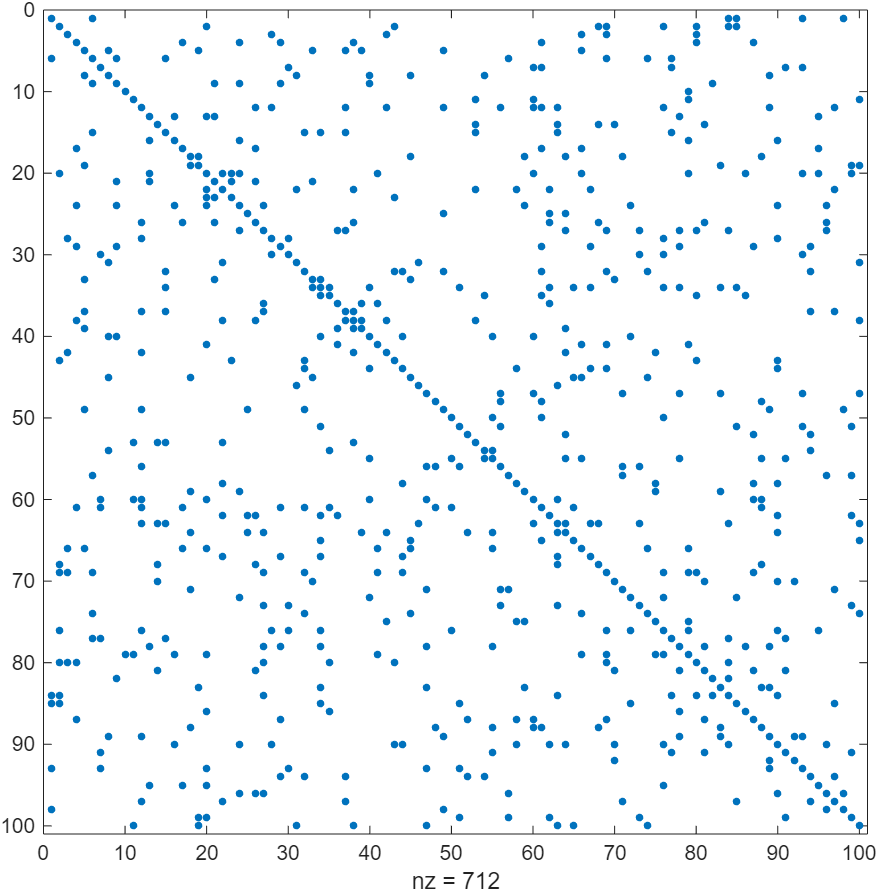
\includegraphics[width=0.5\textwidth]{images/94_spy.png} % Replace with your image filename
    \caption{Sparsità del complementare $A_{94}^C$ della matrice di adiacenza del grafo $A_{94}$ di densità $94\%$. In blu sono indicati gli elementi non nulli
    di $A_{94}^C$ (e quindi quelli nulli di $A_{94}$).}
    \label{fig:spy_94}
\end{figure}

\begin{figure}[H]
    \centering
    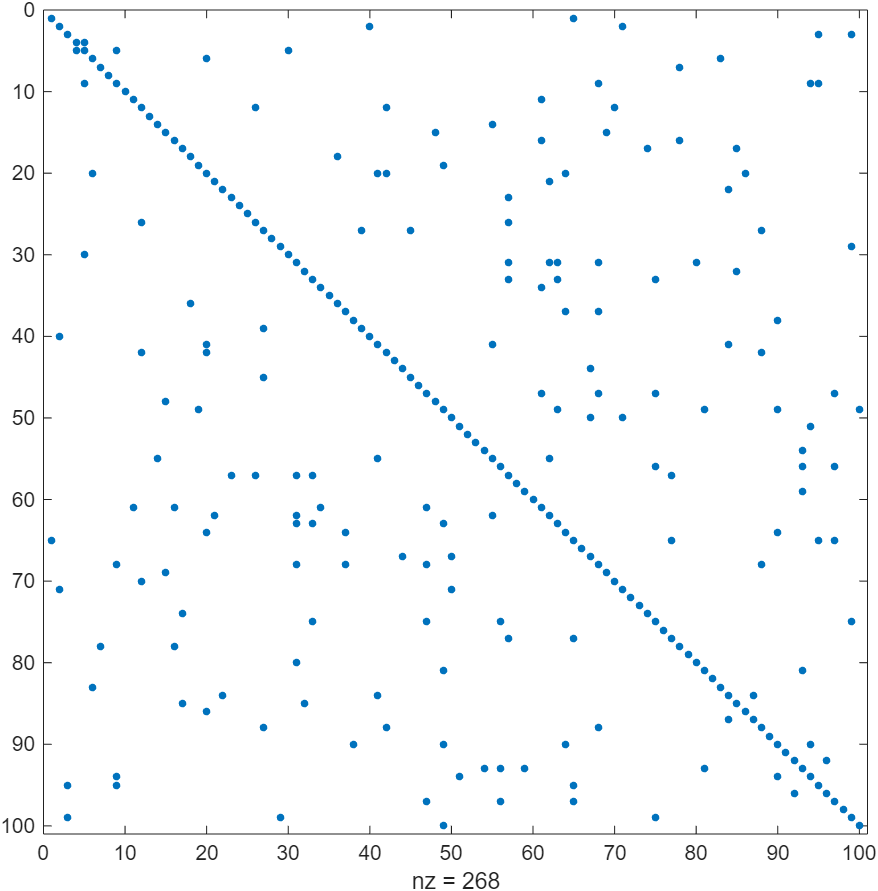
\includegraphics[width=0.5\textwidth]{images/98_spy.png} % Replace with your image filename
    \caption{Sparsità del complementare $A_{98}^C$ della matrice di adiacenza del grafo $A_{98}$ di densità $98\%$. In blu sono indicati gli elementi non nulli
    di $A_{98}^C$ (e quindi quelli nulli di $A_{98}$).}
    \label{fig:spy_98}
\end{figure}

\begin{figure}[H]
    \centering
    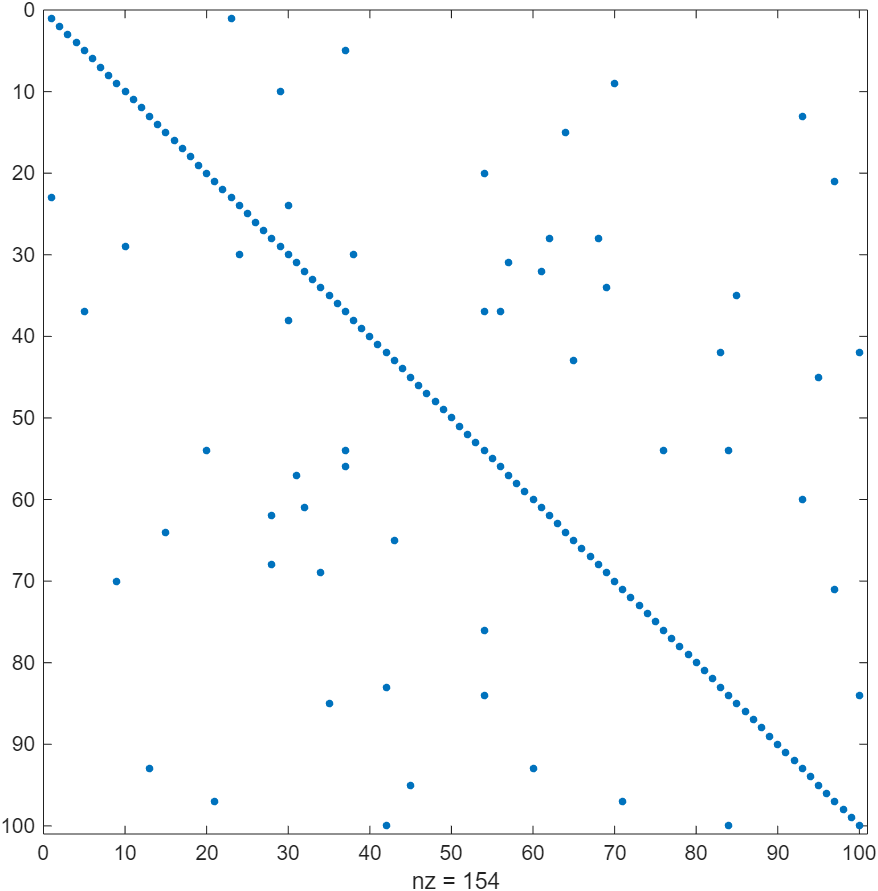
\includegraphics[width=0.5\textwidth]{images/995_spy.png} % Replace with your image filename
    \caption{Sparsità del complementare $A_{99.5}^C$ della matrice di adiacenza del grafo $A_{99.5}$ di densità $99.5\%$. In blu sono indicati gli elementi non nulli
    di $A_{99.5}^C$ (e quindi quelli nulli di $A_{99.5}$).}
    \label{fig:spy_995}
\end{figure}

\subsection{Implementazione degli algoritmi}

Trattandosi di grafi non diretti, per calcolare il vettore di Katz, sia sulla matrice di adiacenza originale, che su quella complementare (con o senza lacci), si è
utilizzato il metodo iterativo MINRES, come illustrato nei Codici \ref{code:katz_classic}, \ref{code:katz_complement} e \ref{code:katz_complement_no_loops}.

\begin{figure}[H]
    \centering
    \begin{lstlisting}[style=Matlab-editor, frame=single, numbers=left, caption={Contenuto del file \texttt{katz\_classic.m}. La funzione risolve iterativamente col metodo MINRES il classico sistema $(I - \alpha A) \xvec = \evec$. I valori restituiti sono il vettore di Katz (\texttt{r}), il tempo impiegato per eseguire il metodo MINRES (\texttt{time}) e il numero di iterazioni del suddetto metodo (\texttt{it}).}, captionpos=b, label=code:katz_classic]
function [r, time, it] = katz_classic(A, alpha, tol, maxit)
    n = size(A, 1);
    I = eye(n);
    
    a = tic;
    [r, ~, ~, it] = minres(I - alpha * A, ones(n,1), tol, maxit);
    time = toc(a);
end      
    \end{lstlisting}
\end{figure}

\begin{figure}[H]
    \centering
    \begin{lstlisting}[style=Matlab-editor, frame=single, numbers=left, caption={Contenuto del file \texttt{katz\_complement.m}. La funzione calcola la matrice di adiacenza complementare \textit{con lacci} $B$ di $A$ e risolve iterativamente col metodo MINRES il sistema $(I + \alpha B) \xvec = \evec$, in accordo al Teorema \ref{th:compl_1}. I valori restituiti sono il vettore di Katz (\texttt{r}), il tempo impiegato per eseguire il metodo MINRES (\texttt{time}) e il numero di iterazioni del suddetto metodo (\texttt{it}).}, captionpos=b, label=code:katz_complement]
function [r, time, it] = katz_complement(A, alpha, tol, maxit)
    n = size(A, 1);
    I = speye(n);
    
    B = sparse(~A);
    
    a = tic;
    [r, ~, ~, it] = minres(I + alpha * B, ones(n,1), tol, maxit);
    time = toc(a);
end       
    \end{lstlisting}
\end{figure}

\begin{figure}[H]
    \centering
    \begin{lstlisting}[style=Matlab-editor, frame=single, numbers=left, caption={Contenuto del file \texttt{katz\_complement\_no\_loops.m}. La funzione calcola la matrice di adiacenza complementare \textit{senza lacci} $B$ di $A$ e risolve iterativamente col metodo MINRES il sistema $\left(I + \frac{\alpha}{1 + \alpha} B\right) \xvec = \evec$, in accordo al Teorema \ref{th:compl_2}. I valori restituiti sono il vettore di Katz (\texttt{r}), il tempo impiegato per eseguire il metodo MINRES (\texttt{time}) e il numero di iterazioni del suddetto metodo (\texttt{it}).}, captionpos=b, label=code:katz_complement_no_loops]
function [r, time, it] = katz_complement_no_loops(A, alpha, tol, maxit)
    n = size(A, 1);
    I = speye(n);
    
    B = sparse(~A);
    B(1 : n+1 : end) = 0;
    
    a = tic;
    [r, ~, ~, it] = minres(I + alpha / (1 + alpha) * B, ones(n,1), tol, maxit);
    time = toc(a);
end       
    \end{lstlisting}
\end{figure}

\subsection{Esperimento sui grafi generati e analisi dei risultati}

Infine si sono eseguite tutte e tre le funzioni presentate per calcolare il ranking di Katz sulle matrici $A_{94}$, $A_{98}$ e
$A_{99.5}$, scegliendo una tolleranza \texttt{tol} pari a $10^{-8}$ e un numero massimo di iterazioni \texttt{maxit} pari a
$1000$. I tempi e i numeri delle iterazioni dell'esperimento (su una media di $30$ esecuzioni per ogni funzione) è
consultabile sulla Tabella \ref{tab:results}. Il codice con cui si è eseguito l'esperimento è consultabile al nome di \texttt{experiment.m}
su \cite{hearotCode}.

\begin{table}[H]
    \centering
    
    \vskip 0.1in
    
    \begin{tabular}{|l|cc|cc|cc|}
        \hline
        \multirow{2}*{$A$} & \multicolumn{2}{|c|}{Codice \ref{code:katz_classic}} & \multicolumn{2}{|c|}{Codice \ref{code:katz_complement}} & \multicolumn{2}{|c|}{Codice \ref{code:katz_complement_no_loops}} \\
                           & iter          & tempo (s)            & iter          & tempo (s)            & iter          & tempo (s)            \\
        \hline
        $A_{94}$ & $4$ & $\approx 9.62 \cdot \mathbf{10^{-1}}$ & $3$ & $\approx 1.99 \cdot \mathbf{10^{-1}}$ & $3$ & $\approx 1.97 \cdot \mathbf{10^{-1}}$ \\
        \hline
        $A_{98}$ & $3$ & $\approx 8.45 \cdot \mathbf{10^{-1}}$ & $3$ & $\approx 6.74 \cdot \mathbf{10^{-2}}$ & $3$ & $\approx 6.77 \cdot \mathbf{10^{-2}}$ \\
        \hline
        $A_{99.5}$ & $3$ & $\approx 8.89 \cdot \mathbf{10^{-1}}$ & $3$ & $\approx 1.93 \cdot \mathbf{10^{-2}}$ & $3$ & $\approx 1.80 \cdot \mathbf{10^{-2}}$ \\
        \hline
    \end{tabular}

    \caption{Numero di iterazioni e tempi di esecuzione per calcolare iterativamente il ranking di Katz su $A_{94}$, $A_{98}$ e $A_{99.5}$ con le funzioni dei Codici \ref{code:katz_classic},
    \ref{code:katz_complement} e \ref{code:katz_complement_no_loops} con tolleranza \texttt{tol} pari a $10^{-8}$ e numero massimo di iterazioni pari
    a $1000$.}
    \label{tab:results}
\end{table}

I risultati predisposti nella Tabella \ref{tab:results} sono totalmente coerenti con le conclusioni di \cite{katz2024}. In tutti e tre i casi,
gli algoritmi indotti dal Teorema \ref{th:compl_1} e \ref{th:compl_2} sono molto più efficienti della risoluzione classica del
Codice \ref{code:katz_classic}. Inoltre, l'efficienza dei Codici \ref{code:katz_complement} e \ref{code:katz_complement_no_loops} migliora notevolmente
all'aumentare della densità delle matrici di input: in linea teorica questo è totalmente comprensibile, dal momento che ciò vorrebbe dire
aumentare la sparsità delle matrici complementari.

\printbibliography

\end{document}